\chapter{Конструкторская часть}


Вычислительный этап конвейера (ОУ2) выполняет обработку графа, полученного из входного файла Graphviz (dot): определяется разбиение вершин на компоненты связности. Для реализации предусмотрены два варианта алгоритма: последовательный обход графа в ширину (BFS) и параллельная обработка рёбер с использованием структуры непересекающихся множеств (DSU) и $k$ вспомогательных потоков.

Схема последовательного алгоритма приведена на рисунке~\ref{fig:cc_seq}, а схема параллельного алгоритма на DSU --- на рисунке~\ref{fig:cc_par}.

\begin{figure}[H]
	\centering
	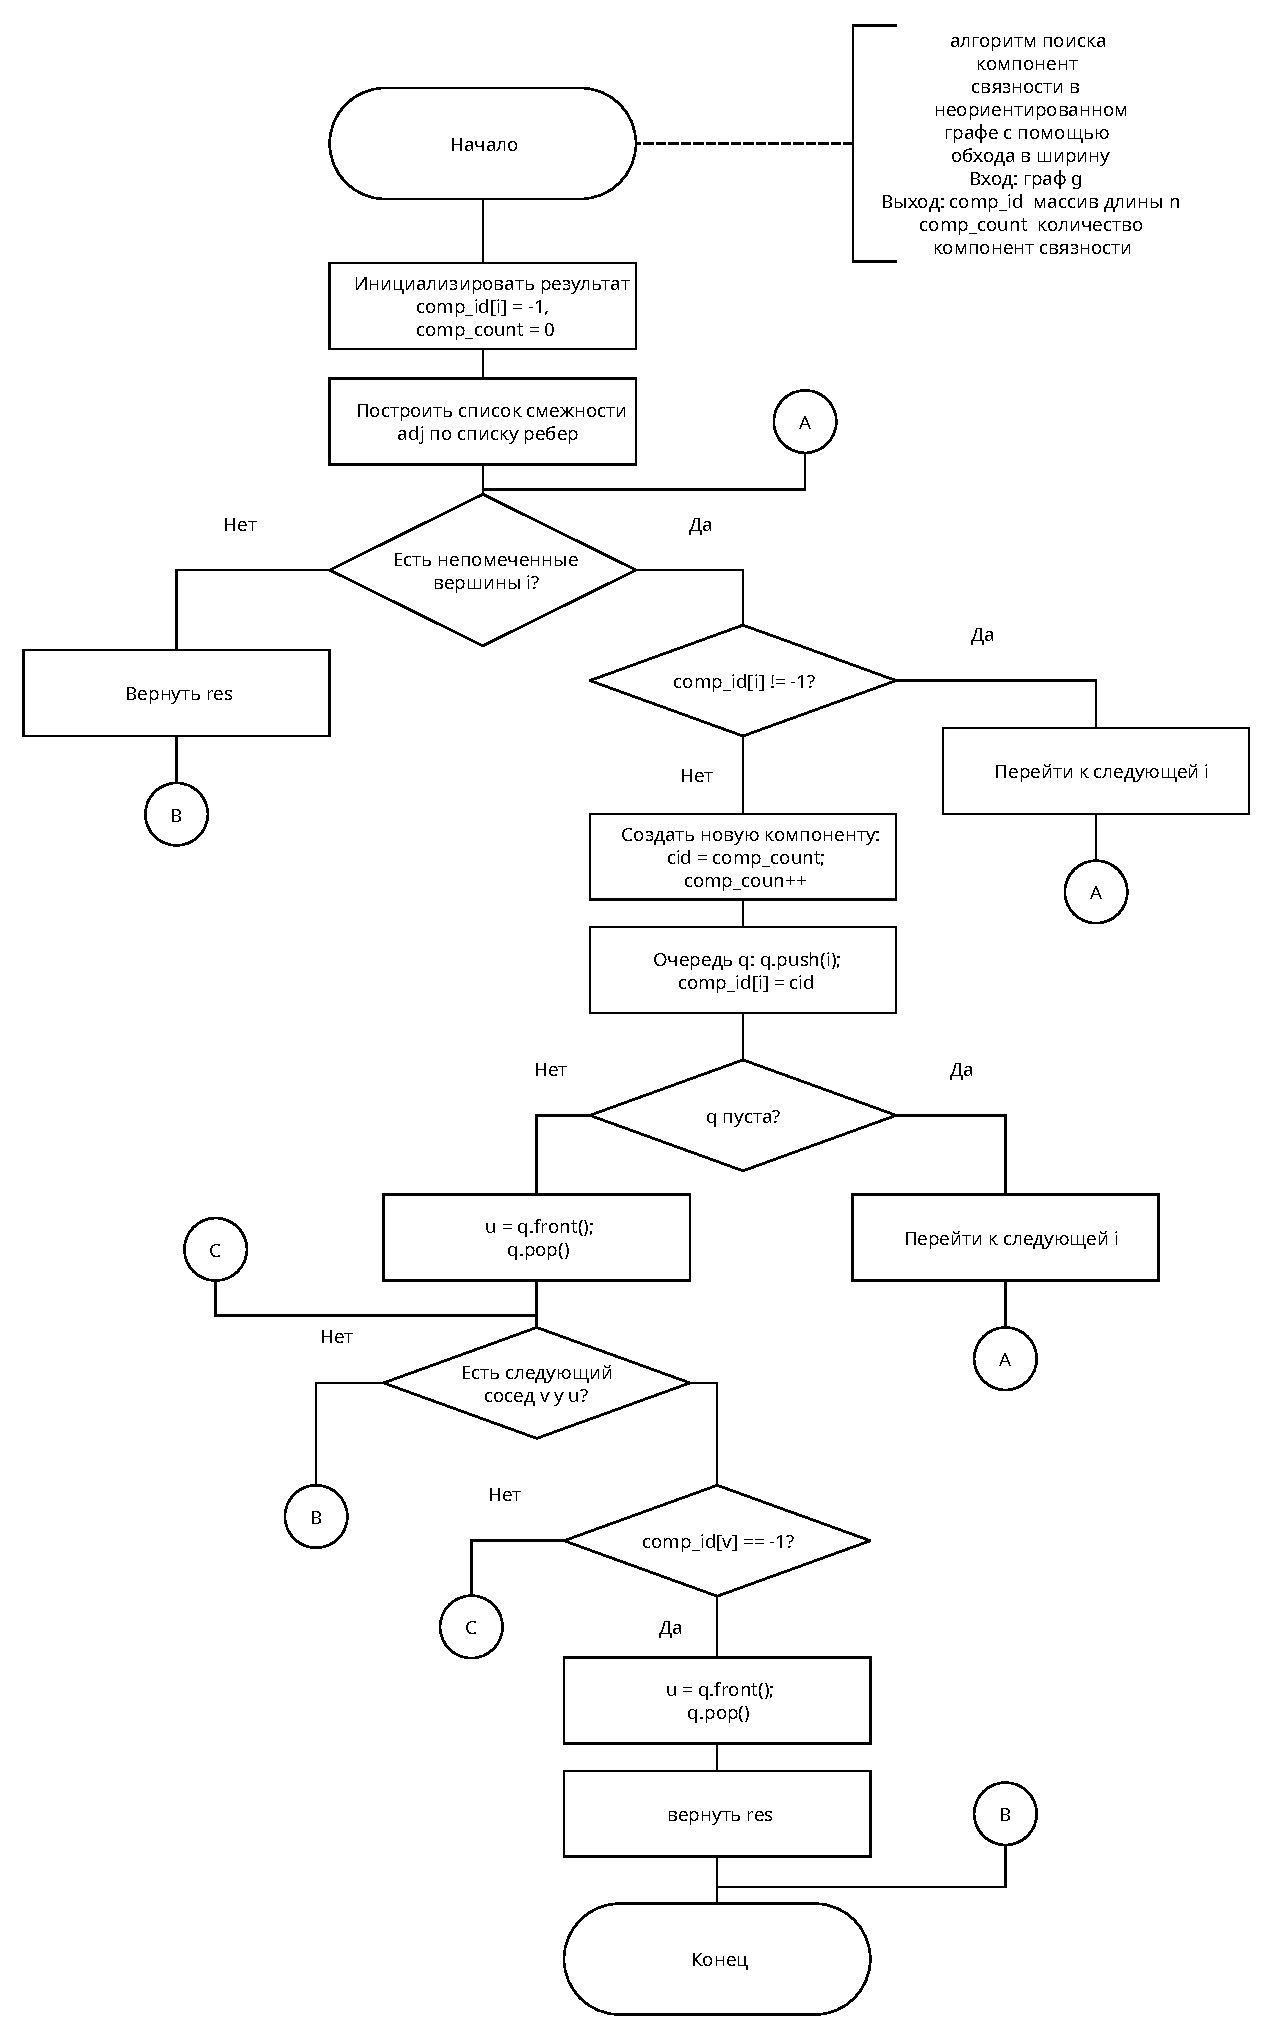
\includegraphics[width=0.82\linewidth]{images/s1.pdf}
	\caption{Блок-схема алгоритма поиска компонент связности (последовательный BFS)}
	\label{fig:cc_seq}
\end{figure}

\begin{figure}[H]
	\centering
	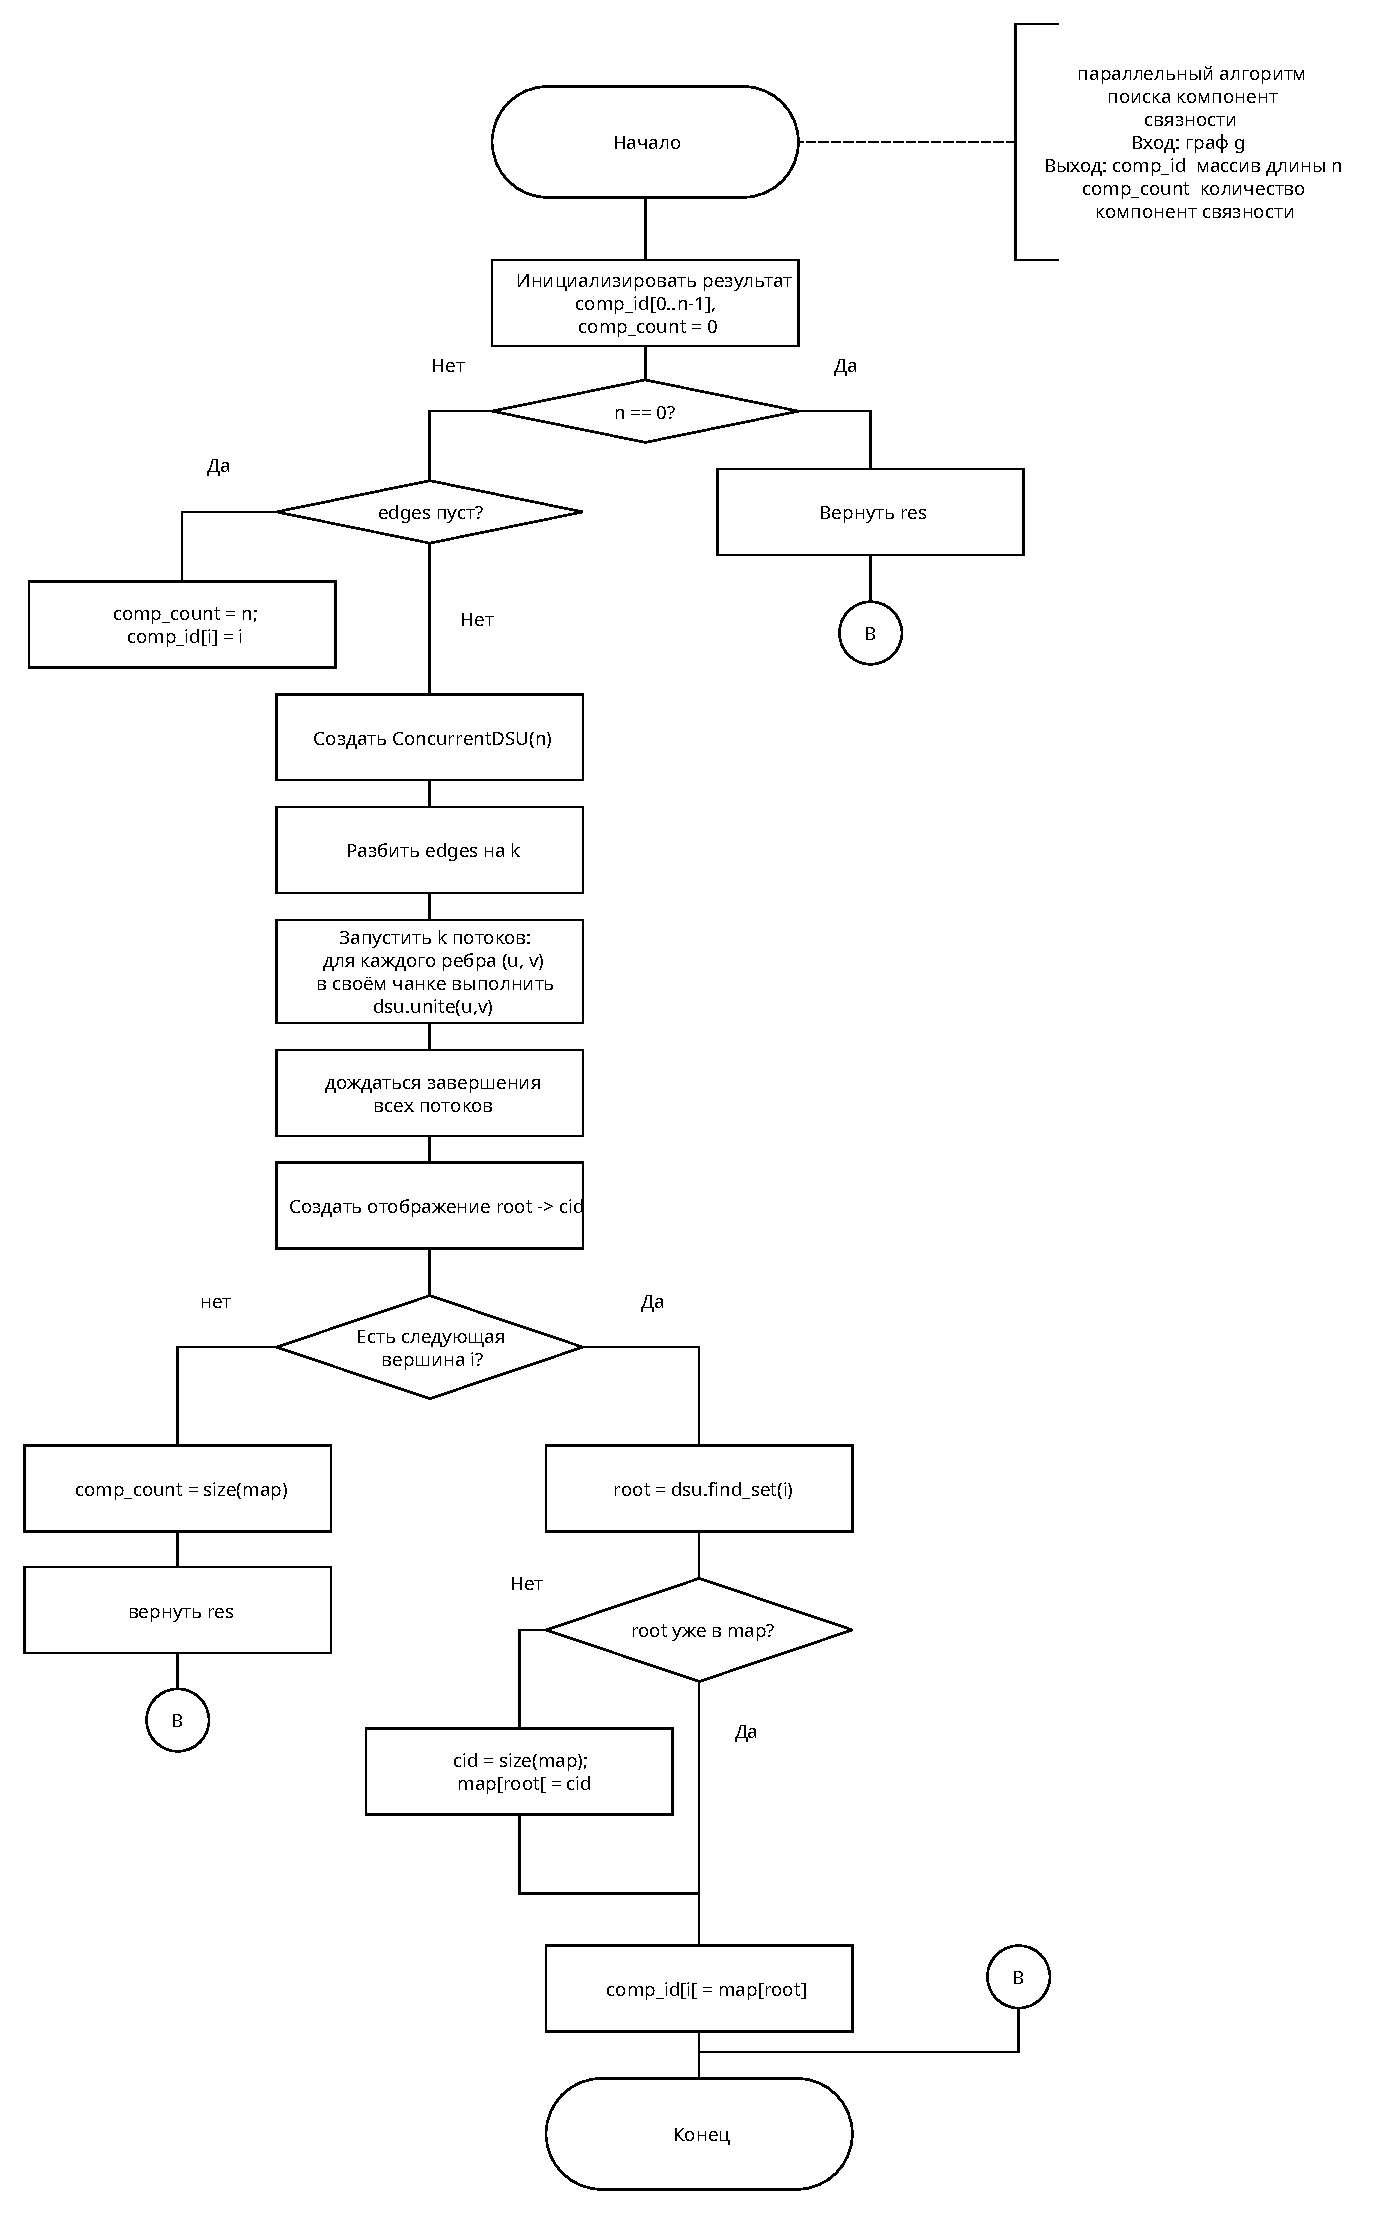
\includegraphics[width=0.92\linewidth]{images/s2.pdf}
	\caption{Блок-схема алгоритма поиска компонент связности (параллельный DSU, $k$ потоков)}
	\label{fig:cc_par}
\end{figure}
